\documentclass[conference]{IEEEtran}
\usepackage{graphicx}
\usepackage{booktabs}
\usepackage{amsmath}
\usepackage{cite}
\usepackage{url}

\begin{document}

\title{SmartWatt: Drift-Aware Adaptive Thresholds and Isolation Forest for Electricity Consumption Anomaly Detection}

\author{\IEEEauthorblockN{Author One, Author Two}
\IEEEauthorblockA{Department of Computer Science, Institution Name\\
City, Country\\
email@example.com}}

\maketitle

\begin{abstract}
Household electricity consumption follows daily and weekly routines and changes slowly over time, so a single global threshold is a poor detector of unusual readings. We present SmartWatt, a software-based anomaly detection pipeline that compares five detectors on hourly consumption data: a fixed-threshold baseline, a time-aware adaptive threshold, a drift-aware online (EWMA) threshold, Isolation Forest, and a hybrid that combines Isolation Forest with the adaptive threshold. All features and baselines use only past observations, and evaluation uses a chronological train/test split with precision, recall, F1-score and false alarm rate. On controlled synthetic data with known anomalies and gradual usage drift, the drift-aware threshold reaches an F1-score of 0.959, against 0.307 for the fixed threshold and 0.428 for Isolation Forest. On the real UCI household dataset, where anomalies are injected because no labels exist, all detectors perform poorly (F1 between 0.157 and 0.239); time-aware adaptive methods are modestly better than the fixed threshold and Isolation Forest, but the hybrid does not outperform the adaptive threshold alone. We report these mixed results, analyse why simple threshold methods struggle on bursty household load, and release the code for reproduction.
\end{abstract}

\begin{IEEEkeywords}
anomaly detection, electricity consumption, Isolation Forest, adaptive threshold, concept drift, smart meters
\end{IEEEkeywords}

\section{Introduction}
Smart meters make fine-grained household consumption data widely available. Unexpected increases or drops can indicate faulty appliances, appliances left on, or outages, and flagging them helps users monitor energy use. Detecting such readings is difficult because ``normal'' depends on the hour of day, the day of week, and the household's changing habits. A fixed global threshold ignores this context: a reading that is ordinary at 19:00 may be highly unusual at 03:00.

Anomaly detection in time series has been surveyed extensively \cite{chandola2009}. Tree-based isolation methods such as Isolation Forest \cite{liu2008} are popular because they need no labels, while robust statistics based on the median and median absolute deviation (MAD) provide outlier scores that are less sensitive to the outliers themselves \cite{leys2013}. Changing usage patterns are an instance of concept drift \cite{gama2014}, which static models do not handle.

This paper is an empirical study. It asks whether combining time-aware adaptive thresholds with Isolation Forest improves detection over each used alone, and whether making the threshold explicitly drift-aware helps further. Our contributions are:
\begin{itemize}
\item an open, reproducible pipeline comparing five detectors under a leakage-free chronological protocol;
\item a drift-aware online threshold that maintains per-slot (hour, day type) baselines using exponentially weighted updates and excludes flagged points from the update;
\item an evaluation on controlled synthetic data with drift and on real household data with injected anomalies, including an honest account of where the methods fail.
\end{itemize}
We do not claim a new algorithm; the components are established, and the contribution is the controlled comparison and its findings.

\section{Related Work}
Chandola et al.\ survey anomaly detection techniques and their assumptions \cite{chandola2009}. Isolation Forest isolates points by random partitioning, assigning shorter average path lengths to anomalies \cite{liu2008}. Leys et al.\ argue for MAD-based outlier criteria over mean and standard deviation \cite{leys2013}, which motivates our robust adaptive score. Gama et al.\ survey adaptation to concept drift \cite{gama2014}. Our work applies these established ideas to household electricity data and evaluates them together. A fuller review of energy-specific anomaly detection literature should be added before submission.

\section{Method}
\subsection{Problem and Features}
Let $x_t$ be the consumption at hour $t$. The goal is a binary label $y_t$ (anomalous or normal) for each reading. For the Isolation Forest we use nine features: the reading $x_t$, $\sin$ and $\cos$ of the hour of day, a weekend indicator, the previous reading $x_{t-1}$, the first difference $x_t - x_{t-1}$, the mean and standard deviation of the previous 24 readings, and the ratio of $x_t$ to that rolling mean. All rolling statistics are computed on past data only.

\subsection{Detectors}
\textbf{Fixed threshold.} A reading is flagged if $|x_t-\mu|>3\sigma$, with $\mu,\sigma$ estimated on the training split.

\textbf{Adaptive threshold.} Readings are grouped by slot $s=(\text{hour},\text{weekend})$. For slot $s$, the baseline $m_t$ is the median of the previous 14 readings in that slot and the scale is $\hat\sigma_t=\max(1.4826\cdot\text{MAD},0.05)$. The score is $z_t=(x_t-m_t)/\hat\sigma_t$ and a reading is flagged if $|z_t|>4$.

\textbf{Drift-aware (EWMA) threshold.} For each slot we keep an exponentially weighted mean $\mu_s$ and mean absolute deviation $d_s$ with rate $\alpha=0.1$. A reading is flagged if $|x_t-\mu_s|>4\cdot\max(1.25\,d_s,0.05)$ once the slot has at least four observations. Flagged readings are not used to update the baseline, preventing anomalies from contaminating it, while unflagged readings move the baseline so that slow changes in usage are tracked.

\textbf{Isolation Forest.} 200 trees, contamination $0.03$, fitted on the training split.

\textbf{Hybrid.} A reading is flagged if $|z_t|>5$, or if Isolation Forest flags it and $|z_t|>2.5$. The adaptive score confirms Isolation Forest alerts, while very large deviations are flagged directly.

\subsection{Evaluation Protocol}
All methods are implemented in Python with scikit-learn \cite{pedregosa2011}.

Each series is split chronologically: the first 60\% is the training period (used to fit the fixed threshold and Isolation Forest) and the last 40\% is the test period. Features and adaptive baselines use only earlier readings, so predicting over the full series gives the test period its history without using future data. We report precision, recall, F1-score and the false alarm rate (FAR), the fraction of normal readings flagged, on the test period.

\section{Experimental Setup}
\subsection{Synthetic Data}
We generate 180 days of hourly consumption with morning and evening peaks, a weekend afternoon peak, a slow seasonal term, multiplicative log-normal noise, and a gradual usage increase of 40\% ramped over days 90--120 to represent concept drift (for example, a new appliance). We inject four types of labelled anomalies, about 3\% of readings: single-hour spikes (2.5--4.5$\times$), sustained high use for 3--6 hours, unusual night use between 00:00 and 04:00, and outage-like drops. Results are averaged over 10 independent datasets.

\subsection{Real Data}
We use the UCI Individual Household Electric Power Consumption dataset \cite{hebrail2006}: one household, December 2006 to November 2010, one-minute resolution. We use Global active power in kW, resample to hourly means and interpolate missing values, giving about 34.6\,k hourly readings. The dataset has no anomaly labels, so we inject labelled anomalies of the same four types with magnitudes scaled to the household's mean consumption (about 3\% of readings). The underlying consumption and its drift are real; only the anomalies are synthetic. We average over 5 independent injection seeds on the same real series; the reported standard deviations therefore reflect injection randomness, not variation across households.

\section{Results}
Tables~\ref{tab:synth} and~\ref{tab:real} give mean $\pm$ standard deviation; the best F1 in each table is in bold.

\begin{table}[t]
\caption{Synthetic data with drift (10 datasets, test period)}
\label{tab:synth}
\centering
\small
\setlength{\tabcolsep}{3pt}
\begin{tabular}{lcccc}
\toprule
Detector & Precision & Recall & F1 & FAR \\
\midrule
Fixed threshold & 0.876$\pm$0.092 & 0.191$\pm$0.089 & 0.307$\pm$0.125 & 0.001$\pm$0.001 \\
Adaptive threshold & 0.755$\pm$0.111 & 1.000$\pm$0.000 & 0.856$\pm$0.082 & 0.011$\pm$0.003 \\
\textbf{Drift-adaptive (EWMA)} & \textbf{0.923$\pm$0.060} & \textbf{1.000$\pm$0.000} & \textbf{0.959$\pm$0.034} & \textbf{0.003$\pm$0.002} \\
Isolation Forest & 0.496$\pm$0.119 & 0.409$\pm$0.118 & 0.428$\pm$0.080 & 0.018$\pm$0.013 \\
Hybrid adaptive & 0.832$\pm$0.062 & 0.986$\pm$0.011 & 0.901$\pm$0.035 & 0.006$\pm$0.002 \\

\bottomrule
\end{tabular}
\end{table}

\begin{table}[t]
\caption{Real UCI data with injected anomalies (5 injection seeds, test period)}
\label{tab:real}
\centering
\small
\setlength{\tabcolsep}{3pt}
\begin{tabular}{lcccc}
\toprule
Detector & Precision & Recall & F1 & FAR \\
\midrule
Fixed threshold & 0.574$\pm$0.064 & 0.091$\pm$0.019 & 0.157$\pm$0.030 & 0.002$\pm$0.000 \\
Adaptive threshold & 0.153$\pm$0.008 & 0.457$\pm$0.028 & 0.229$\pm$0.012 & 0.090$\pm$0.001 \\
\textbf{Drift-adaptive (EWMA)} & \textbf{0.190$\pm$0.012} & \textbf{0.323$\pm$0.015} & \textbf{0.239$\pm$0.013} & \textbf{0.049$\pm$0.001} \\
Isolation Forest & 0.373$\pm$0.077 & 0.140$\pm$0.028 & 0.203$\pm$0.041 & 0.008$\pm$0.001 \\
Hybrid adaptive & 0.164$\pm$0.009 & 0.410$\pm$0.028 & 0.234$\pm$0.013 & 0.075$\pm$0.001 \\

\bottomrule
\end{tabular}
\end{table}

\begin{figure}[t]
\centering
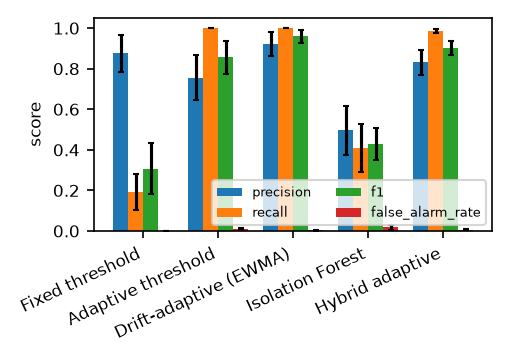
\includegraphics[width=\columnwidth]{fig_synth_bar.png}
\caption{Metrics on synthetic data with drift (mean $\pm$ std over 10 datasets).}
\label{fig:synth}
\end{figure}

\begin{figure}[t]
\centering
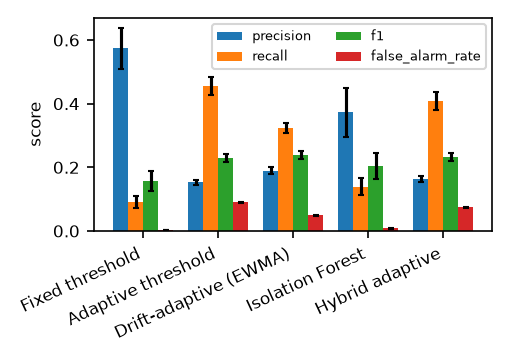
\includegraphics[width=\columnwidth]{fig_real_bar.png}
\caption{Metrics on real UCI data with injected anomalies (mean $\pm$ std over 5 injection seeds).}
\label{fig:real}
\end{figure}

\begin{figure}[t]
\centering
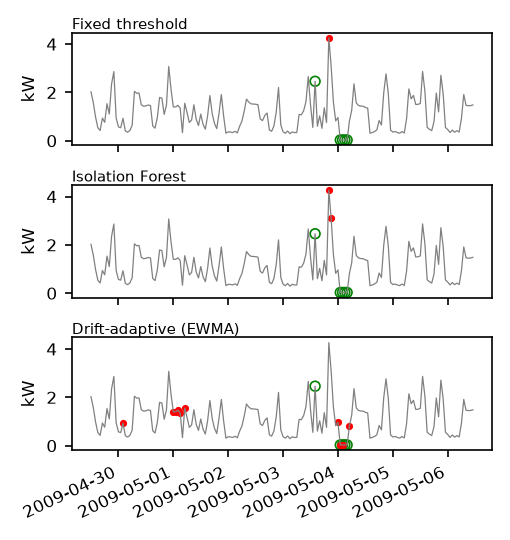
\includegraphics[width=\columnwidth]{fig_det_real.png}
\caption{One week of the real test period. Gray: consumption; green circles: injected anomalies; red dots: flagged readings.}
\label{fig:det}
\end{figure}

\subsection{Synthetic data}
The drift-aware threshold achieves the best F1 (0.959), with perfect recall and few false alarms. The static 14-day adaptive threshold (0.856) and the hybrid (0.901) are clearly better than the fixed threshold (0.307), which misses most anomalies that are unusual only for their time of day, and than Isolation Forest alone (0.428), which lacks slot-specific context and is hurt by the usage shift. Here the hybrid improves on both the adaptive threshold and Isolation Forest, consistent with the hypothesis, but is itself outperformed by the drift-aware threshold.

\subsection{Real data}
Performance drops sharply on real data (Table~\ref{tab:real}). The best F1 is only 0.239 (drift-aware), followed by the hybrid (0.234), the adaptive threshold (0.229), Isolation Forest (0.203) and the fixed threshold (0.157). The three time-aware methods are within about one standard deviation of each other (no significance test was run) and the hybrid brings no benefit over the adaptive threshold alone. They do improve recall (0.32--0.46 versus 0.09 for the fixed threshold) but at a false alarm rate of 4.9--9.0\%, against 0.2\% for the fixed threshold. The fixed threshold and Isolation Forest are conservative, with higher precision but low recall. Raising the threshold factor did not help: selecting the factor on the training period alone returned the default value of 4.

\subsection{Why real data is harder}
Household load is bursty. Appliance events such as kettles, ovens and heaters create large, short, irregular peaks, so the normal range for a given slot is wide and heavy-tailed. Many injected anomalies, especially additive increases at the household's mean scale, lie inside that range and are indistinguishable from legitimate use by a per-slot threshold. This reflects a genuine limit of univariate threshold methods and suggests that per-appliance sub-metering or longer-window features are needed.

\section{Limitations}
\begin{itemize}
\item The synthetic generator contains exactly the daily, weekly and drift structure the adaptive methods exploit, so synthetic results favour them.
\item Real-data anomalies are injected, not naturally occurring; results depend on the injection recipe and magnitude, and detectors may behave differently on true faults.
\item Only one household is used, and the standard deviations on real data reflect injection randomness only.
\item Hyperparameters (thresholds 3, 4 and 5, 2.5, window 14, $\alpha=0.1$) were set a priori. Only the threshold factor was checked on the training period for the real data; a full validation-based search was not performed.
\item The comparison omits stronger baselines such as seasonal-decomposition residuals, autoencoders, or LSTM forecasters.
\end{itemize}

\section{Conclusion}
We compared fixed, adaptive, drift-aware, Isolation Forest and hybrid detectors for electricity anomaly detection. With clear routines and gradual drift, a drift-aware time-adaptive threshold substantially outperforms a fixed threshold and Isolation Forest. On real, bursty household data, all methods perform poorly, with time-aware adaptive methods only modestly ahead, and combining them with Isolation Forest adds no measurable benefit over the adaptive threshold alone. Future work includes validation-based tuning, multi-hour window features, stronger baselines, multiple households, and evaluation against genuinely labelled faults.

\section*{Reproducibility}
Code, the experiment scripts and a notebook are available in the project repository (add a public link before submission).

\begin{thebibliography}{00}
\bibitem{chandola2009} V. Chandola, A. Banerjee, and V. Kumar, ``Anomaly detection: A survey,'' \emph{ACM Computing Surveys}, vol. 41, no. 3, pp. 1--58, 2009.
\bibitem{liu2008} F. T. Liu, K. M. Ting, and Z.-H. Zhou, ``Isolation forest,'' in \emph{Proc. IEEE Int. Conf. Data Mining (ICDM)}, 2008, pp. 413--422.
\bibitem{leys2013} C. Leys, C. Ley, O. Klein, P. Bernard, and L. Licata, ``Detecting outliers: Do not use standard deviation around the mean, use absolute deviation around the median,'' \emph{J. Experimental Social Psychology}, vol. 49, no. 4, pp. 764--766, 2013.
\bibitem{gama2014} J. Gama, I. \v{Z}liobait\.{e}, A. Bifet, M. Pechenizkiy, and A. Bouchachia, ``A survey on concept drift adaptation,'' \emph{ACM Computing Surveys}, vol. 46, no. 4, pp. 1--37, 2014.
\bibitem{hebrail2006} G. Hebrail and A. Berard, ``Individual household electric power consumption,'' UCI Machine Learning Repository, 2006. [Online]. Available: \url{https://archive.ics.uci.edu/dataset/235}
\bibitem{pedregosa2011} F. Pedregosa \emph{et al.}, ``Scikit-learn: Machine learning in Python,'' \emph{J. Machine Learning Research}, vol. 12, pp. 2825--2830, 2011.
\end{thebibliography}

\end{document}
